%
% chap002.tex
%

\chapter{Satz von Wilson}

In diesem Abschnitt der Arbeit werden die ausführlichen Daten
hinsichtlich des Satzes, die Mathematiker, die sich mit dem
Satz von Wilson beschäftigt haben, in den Vordergrund gebracht,
und einige Beweise dieses Satzes näher vorgestellt. Des Weiteren
werden kurze Berechnungen bezüglich des Satzes betrachtet.
\vspace{.2cm}

%======================================================
\section{Satz von Wilson}
%======================================================

Der Satz von Wilson kann auf zwei Varianten definiert werden.
Die eine Variante, bei der Kongruenz nicht einbezogen ist,
kommt selten in den Literaturen vor, wobei diese Variante -
auch bei der Berechnung - viel einfacher zu verstehen ist.
Hauptsächlich und in den meisten Büchern und Skripten ist die
zweite Variante inklusive der Kongruenz zu sehen. Des Weiteren
wird die zweite Variante je nach Autor des Buches oder Skripts
unterschiedlich formuliert, wobei alle Formulierungen
gleichwertig sind. In den weiteren Paragrafen werden beide
Arten des Satzes vorgestellt.

\begin{theorem}[Satz von Wilson]
``Wenn $p$ eine Primzahl ist, dann ist $1 +(p-1)!$ durch
$p$ teilbar'' (O'Connor \& Robertson, 2005).
\end{theorem}

\begin{theorem}[Satz von Wilson]
``Es ist $p$ genau dann eine Primzahl, wenn
$(p-1)! \;\equiv\; -1\mod p$''
(Rechnen mit Restklassen, 2021).
\end{theorem}

Außerdem gibt es eine weitere Option des Satzes, nämlich
die Umkehrung. Diese lautet:

\begin{theorem}[Umkehrung des Satzes von Wilson]
``Wenn $n$  $1+(n-1)!$ teilt, dann ist $n$ eine Primzahl''
(vgl. O'Connor \& Robertson, 2005).
\end{theorem}

Der Satz von Wilson wurde zuerst von dem arabischen
Mathematiker Abu Ali al-Hasan ibn al-Haytham, im
Deutschen unter Alhazen bekannt, entdeckt und er wurde
mehr als 700 Jahre später von John Wilson wiederentdeckt
(vgl. Foco 2009, S.3 \& vgl. Alhazen, 2021). Jedoch konnten
beide Mathematiker den Satz nicht beweisen
(vgl. O'Connor \& Robertson, 2005 \& vgl. Ziegenbalg 2015,
S.116). Der Satz und die Umkehrung wurden erstmals
vollständig im Jahr 1773 von Lagrange bewiesen
(vgl. Ziegenbalg 2015, S. 116).


%======================================================
\section{Abu Ali al-Hasan ibn al-Haytham}
%======================================================

\begin{minipage}{0.65\linewidth}
Der arabische Wissenschaftler Abu Ali al-Hasan Ibn al-Ha-
ytham, abgekürzt Ibn al-Haytham und im Deutschen unter
Alhazen bekannt, war ein engagierter Mathematiker,
Physiker, Astronom (vgl. Rashed, 2021). Geboren ist
Alhazen um 965 n. Chr. in Basra (im heutigen Iraq) und
er beschäftigte sich neben der Mathematik insbesondere 
mit der Optik (vgl. Alhazen, 2021 \& vgl. O'Connor \& 
Robertson, Abu Ali al-Hasan ibn al-Haytham, 1999).
Aufgrund seiner bedeutenden wissenschaftlichen Beiträge
hinsichtlich der Optik wurde er auch der ``Vater der Optik''
genannt. Beispielsweise war er der Entdecker der Lupe 
und somit der Mikroskopie (vgl. Alhazen, 2021).
\end{minipage}
\hfil
\begin{minipage}[r]{0.3\linewidth}
  % insert this 2 lines before \includegraphics to avoid the warning "the option `hypcap=true' will be ignored for this particular \caption on input line.
  % This warning occurs, because a conflict at paramter "hypcap=true" when load both packages "hyperref" and "caption".
  %\captionsetup[figure]{labelformat=empty}% turn off figure prefix "Figure:" or "Abbildung"
  \captionsetup{type=figure,font=small,skip=6pt,format=plain}% {format=hand}
  \capstart
  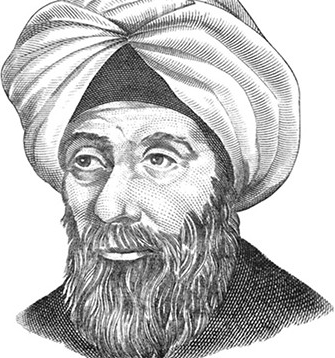
\includegraphics[width=1.0\linewidth]{./images/alhazen.jpg}
  \captionof{figure}[Ibn al-Haytham (Ibn al-Haytham's scientific method, 2015)]{Ibn al-Haytham}
  \label{fig:portrait_alhazen}
\end{minipage}
\vspace{.3cm}

In vielen Literaturen ist Alhazen für seine bedeutenden
optischen Experimente und Arbeiten bekannt. Eine seiner
wichtigen Leistungen war die Forschung hinsichtlich der
``Sehstrahlen''. Die bekannten Wissenschaftler wie Euklid
und Ptolemäus sind damals davon ausgegangen, dass die
sogenannten ``Sehstrahlen'', die das menschliche Auge
verlassen sollten, die Umgebung anfühlten bzw. abtasteten
und so zur Erzeugung des visuellen Eindrucks im Gehirn
führten. Alhazen begann mit seiner Forschung bezüglich
der ``Sehstrahlen'' mit der genauen Untersuchung des
Aufbaues des Auges. Infolgedessen entdeckte er die
Wichtigkeit bzw. die Bedeutung der Linse im Auge und
aufgrund dessen konnte er anhand wissenschaftlicher
Experimente die ``Sehstrahlen''-Theorie widerlegen
(vgl. Alhazen, 2021).

Bezüglich der Mathematik fokussierte sich Alhazen
besonders auf die Geometrie und er schrieb sämtliche
Bücher hinsichtlich dieses mathematischen Gebietes.
Beispielsweise untersuchte er das Problem der Quadratur
des Kreises und die Theorie der Kegelschnitte
(vgl. O'Connor \& Robertson, Abu Ali al-Hasan ibn 
al-Haytham, 1999 \& vgl. Rashed, 2021). Des Weiteren
konnte er anhand seiner Ergebnisse über die Summation
von Potenzen natürlicher Zahlen die Rauminhalte von
Rotationskörpern berechnen (vgl. Ziegenbalg 2015, S. 13).

Außerdem beschäftigte sich Alhazen mit der Zahlentheorie
und entdeckte den nach John Wilson benannten Satz.
Anhand dieses Satzes löste Alhazen die Probleme mit
Kongruenzen und der Satz lautet: wenn $p$ eine Primzahl
ist, dann ist $1+(p-1)!$ durch $p$ teilbar.

Alhazen konnte den Satz jedoch nicht beweisen
(vgl. O'Connor \& Robertson, Abu Ali al-Hasan
ibn al-Haytham, 1999).


%======================================================
\section{John Wilson}
%======================================================

\begin{minipage}{0.65\linewidth}
John Wilson, geboren am 06. August 1741 in Applethwaite,
war ein englischer Mathematiker und Jurist, der für den
nach ihm benannten Satz in der Geschichte der Mathematik
bekannt ist. Studiert hat Wilson von 1757 bis 1761 in
Cambridge und beendete sein Mathematikstudium mit
erfolgreichen Noten. Genauer beschrieben, besaß Wilson
die besten Noten unter den Studenten. Des Weiteren
lehrte Wilson ab 1764 Mathematik in Cambridge und zwei
Jahre später wurde Wilson in die Anwaltskammer berufen
und hörte somit mit der Universitätslehre auf
(vgl. O'Connor \& Robertson, John Wilson, 2005).
\end{minipage}
\hfil
\begin{minipage}[r]{0.3\linewidth}
  % insert this 2 lines before \includegraphics to avoid the warning "the option `hypcap=true' will be ignored for this particular \caption on input line.
  % This warning occurs, because a conflict at paramter "hypcap=true" when load both packages "hyperref" and "caption".
  %\captionsetup[figure]{labelformat=empty}% turn off figure prefix "Figure:" or "Abbildung"
  \captionsetup{type=figure,font=small,skip=6pt,format=plain}% {format=hand}
  \capstart
  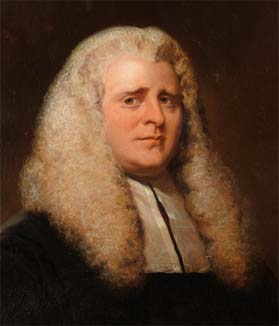
\includegraphics[width=1.0\linewidth]{./images/john_wilson.jpeg}
  \captionof{figure}[John Wilson (John Wilson (mathematician), 2020)]{John Wilson}
  \label{fig:portrait_wilson}
\end{minipage}
\vspace{.3cm}

Wie es im ersten Absatz beschrieben ist, ist John Wilson
unter den Mathematikern für seinen Satz berühmt, den er
1770 wiederentdeckte, da dieser Satz mehr als 700 Jahre
davor von Alhazen zuerst erfunden worden ist
(vgl. Foco 2009, S. 3). John Wilson hat die Vermutung
getroffen, dass die Aussage ``wenn $p$ eine Primzahl ist,
dann ist $1+(p-1)!$ durch $p$ teilbar'' tatsächlich
existiert, jedoch konnte er keinen Beweis für diese
Aussage bzw. für diesen Satz verfassen (vgl.
O'Connor \& Robertson, John Wilson, 2005).

Auch Wilsons Professor Waring konnte den Satz nicht
beweisen, jedoch wurde der Satz von ihm veröffentlicht
und nach Wilson benannt (vgl. O'Connor \& Robertson,
John Wilson, 2005). Im Jahr 1773 bewies Lagrange
erstmals diesen Satz (vgl. Ziegenbalg 2015, S. 116).


%======================================================
\section{Der Beweis des Satzes von Wilson}
%======================================================

Der Satz von Wilson wird in vielen Büchern und Skripten
gleichwertig, aber verschieden formuliert. Aus diesem
Grund gibt es auch viele verschiedene Beweise.
In diesem Unterkapitel der Arbeit möchte ich zwei
Formulierungen des Satzes und die dazugehörigen Beweise
vorstellen.

Einer von vielen Beweisen ist im Buch namens
``Algorithmische Zahlentheorie'' von Otto Forster
(2. Auflage) vorgestellt. Dieser Beweis ist im Vergleich
zu den anderen Beweisen etwas kurz, jedoch nach meiner
Ansicht verständlich erklärt worden. Wie im ersten 
Paragrafen erwähnt ist, ist der Satz in dem Buch
gleichwertig, aber anders definiert.

\begin{theorem}[Wilson]
``Eine natürliche Zahl $p \geq 2$ ist genau dann eine
Primzahl, wenn $(p-1)! \;\equiv\; -1 \mod p$''
(Forster 2015, S. 56).
\end{theorem}
\vspace{-.7cm}

\begin{proof}
 ``Sei $p$ keine Primzahl, sondern besitze einen Teiler
 $q$ mit $1 < q < p$. Dann ist auch $(p-1)!$ durch $q$
 teilbar, also nicht teilerfremd zu $p$. Aber $-1$ ist
 teilerfremd zu $p$, Widerspruch!'' (Forster 2015, S. 56).
\end{proof}

Des Weiteren wurde ein längerer Beweis hinsichtlich
des Satzes von Wilson von Gábor Sas in seiner Arbeit
präsentiert worden.

\begin{theorem}[Wilson]
``$(p-1)! \;\equiv\; -1\mod p\;$ gilt dann und nur dann,
wenn $p$ eine Primzahl ist'' (Sas 2002-2008, S.12f).
\end{theorem}
\vspace{-.7cm}

\begin{proof}
  Dieser Beweis wird in zwei Schritten geführt.
  \begin{itemize}
    \item $p$ prim $\;\Rightarrow\;$ $(p-1)! \;\equiv\; -1 \mod p$\\
          Das Produkt über alle Elemente der multiplikativen Gruppe
          des Körpers $\mathbb{Z}_{p}$ steht links. ``Da mit jedem
          $a \in \mathbb{Z}_{p}^{\star}$ auch
          $a^{-1}\in\mathbb{Z}_{p}^{\star}$ ist, lassen sich die
          Faktoren zu Paaren $a\cdot a^{-1} = 1$ zusammenfassen
          mit Ausnahme der Elemente, welche zu sich selbst invers
          sind, d.h. $a^2 = 1$ erfüllen''. Aufgrund dass die
          Gleichung $x^2 = 1$ im Körper $\mathbb{Z}_{p}$ genau
          die Lösung $\pm 1$ hat, folgt somit die Behauptung
          (vgl. Sas 2002-2008, S.12f).
          
    \item $(p-1)! \;\equiv\; -1\mod p$ $\;\Rightarrow\;$ $p$ prim\\
          ``Ist $p=n\cdot m$, wobei $n$ und $m$ echte Teiler von $p$
          mit $m \neq n$ sind, dann sind beide Faktoren in
          $(p-1)!$ vorhanden und damit ist $(p-1)!$ durch $m\cdot n$
          teilbar, also ist $(p-1)! \;\equiv\; 0 \mod p$.
          Sei nun $p=c^2$ , so ist
          $(p-1)! = (p-1)\cdot (p-2)\cdot \dotsc \cdot (2c)\cdot \dotsc
          \cdot c \cdot \dotsc \cdot 2 \cdot 1$.
          Ist nun $(p-1) > 2c = 2\sqrt{p}$,
          dann enthält $(p-1)!$ mindestens zweimal den Faktor $c$,
          und damit gilt auch $(p-1)! \;\equiv\; 0 \mod p$.
          Die Ungleichung $(p-1) > 2c = 2 \sqrt{p}$ ist für alle
          $p \geq 6$ erfüllt, da $6 − 1 > 2 \sqrt{6} \approx 4,9$
          und die linke Seite wächst schneller als die rechte.
          Damit ist die einzige noch zu behandelnde Quadratzahl
          die $4$, für $p = 4$ gilt jedoch $(p-1)! \;\equiv\;
          3! \;\equiv\; 6 \;\equiv\; 2 \mod 4$''
          (Sas 2002-2008, S 12).
  \end{itemize}
\end{proof}

Somit sind der Satz und die Beweise von zwei unterschiedlichen
Autoren bzw. Verfassern auch unterschiedlich beschrieben.
Es gibt jedoch viele weitere Formulierungen hinsichtlich dieses
Satzes und der Beweise, jedoch werden nur diese in dieser Arbeit
in den Vordergrund gebracht.
